

% PLEASE USE UTF-8 ENCODING WHEN EDITING THIS FILE!

% WWW 2012 page limit: 10 pages

%\documentclass{llncs}
% \documentclass{acm_proc_article-sp}
\documentclass{sig-alternate}  % tighter style --> less pages (use the other one if we have enough space)
%\documentclass{www2012-accepted} 
%\usepackage{amsmath, amssymb}
%\usepackage{graphicx}
\usepackage{hyperref}
%\usepackage{listings}
\usepackage[utf8]{inputenc}
\usepackage{moreverb}
\usepackage{listings}
\usepackage{graphicx}
\usepackage{caption}
\usepackage{subcaption}

\newcommand{\todo}[1]{\textbf{ToDo: \textit{#1}}}
%\newcommand{\comm}[1]{\textbf{Comment: \textit{#1}}}\stackrel{\leftrightarrow}{}

\usepackage{enumitem}
\usepackage[usenames,dvipsnames]{color}
\newcommand{\sparqlwo}[2]{{\texttt{#1 \char '173} \\[1.5pt] \hspace*{.5cm}\parbox{6cm}{\tt #2} \\ \texttt{\char '175} }}
\newcommand{\sparql}[3]{{\texttt{#1 \char '173} \\[1.5pt] \hspace*{.5cm}\parbox{6cm}{\tt #2} \\ \texttt{\char '175} \\ \texttt{#3} }}
\newcommand{\slot}[3]{$\langle\texttt{#1},\text{#2},\text{\sf #3}\rangle$}
\newcommand{\argmax}{\operatornamewithlimits{arg\,max}}
\newcommand{\argmin}{\operatornamewithlimits{arg\,min}}

\usepackage{qtree}
\usepackage[usenames,dvipsnames,table]{xcolor}


\newcommand{\Drs}[2]{%%%%%%%%%%%%%%%%%%%%%%%%%
\(                   % begin maths mode
 \begin{array}{|l|}  %
 \hline              % top line
   \begin{array}{l}  %
    #1                % `Universe'
    \end{array} \\   %  end the `universe' part
 \hline              % line between Universe and Conditions
    \begin{array}{l} %
    #2                % the conditions
    \end{array} \\   % end the conditions part
 \hline              % bottom line
\end{array}          %
\)                   % end maths mode
                     }%%%%%%%%%%%%%%%%%%%%%%%%%


\begin{document}

\clubpenalty=10000 
\widowpenalty = 10000

%\conferenceinfo{WWW}{2012 Lyon, France}

\title{Duplicate-Aware Federated Query Processing over the Data Web}

\numberofauthors{2} 
\author{
% 1st. author
\alignauthor
Muhammad Saleem\\
       \affaddr{Digital Enterprise Research Institute,}\\
       \affaddr{National University of Ireland, Galway}\\ 
       \email{muhammad.saleem@deri.org}
% 2nd. author
\alignauthor
Axel-Cyrille Ngonga Ngomo\\
       \affaddr{Universit\"at Leipzig, IFI/AKSW}\\
       \affaddr{PO 100920, D-04009 Leipzig}\\
       \email{ngonga@informatik.uni-leipzig.de}
}

%\date{30 July 1999}
\maketitle

%\title{SPARQL Template Based Question Answering}
% \titlerunning{SPARQL Template Based Question Answering}  
%\author{Christina Unger\inst{1} \and Lorenz B{\"u}hmann\inst{2} \and Jens Lehmann\inst{2} \and Philipp Cimiano\inst{1}}
%\authorrunning{...} 
%\institute{
%Bielefeld University, CITEC, Semantic Computing Group\\
%Universit\"atsstra{\ss}e 21--23, 33615 Bielefeld\\ 
%\email{cunger|cimiano@cit-ec.uni-bielefeld.de}
%\and 
%University of Leipzig, Computer Science Institute, AKSW Group,
%\\Johannisgasse 26, 04103 Leipzig\\
%\email{buehmann|lehmann@informatik.uni-leipzig.de}
%}
\begin{abstract}
Over the last years, the Linked Data Web has developed into a large compendium of interlinked data sets from diverse domains.
Due to this distributed character, several of these data sets contain either duplicate or complementary data. 
So far, several federated querying approaches have been developed to retrieve information from these data sources.
Still, only little attention has been paid to the effect of duplicates and fragmented data on the ranking of data sources during the processing of federated queries.
This work presents a novel approach federated querying based on min-wise independent permutation vectors applied to RDF predicates.
Our approach allows evaluating the ranking of data sources accurately while taking into account duplicate data.
By these means, our approach achieves significantly smaller mean squared errors that the state of the art with respect to the approximation of result set sizes as well as in the ranking of data sources. 
 \end{abstract}

% A category with the (minimum) three required fields
\category{H.2.4}{Database Management}{Systems}[Distributed databases]
%A category including the fourth, optional field follows...
% \category{D.2.8}{Software Engineering}{Metrics}[complexity measures, performance measures]

\terms{Algorithms, Experimentation, Theory}

\keywords{Federated queries, SPARQL, deduplication}

\section{Introduction (AN+MS)}
Over the last years, the Linked Data Web has developed into a large compendium of interlinked data sets from diverse domains. 
One of the central principles underlying the architecture of these data sets is the reuse of URIs and vocabularies as well as the linking of knowledge bases.
One of the results of this architectural choice is that certain queries can only be answered by retrieving information from several knowledge bases.
This type of querying, called \emph{federated querying}, is of central importance for manifold applications such as question answering, knowledge retrieval and data integration.
In addition to the information necessary to answering queries being distributed, certain pieces of information (i.e., triples) can be found in several knowledge bases. 
For example, the name of movie directors can be found both in DBpedia and LinkedMDB.
Similarly, the authors of papers can be found in both the ACM and DBLP libraries.
We call triples that can be found in several knowledge bases across the Web of Data \emph{duplicates}.

While the importance of federated queries over the Web of Data has been stressed in previous work, the impact of duplicates has not received much attention.
Yet (as we will show in the remainder of this paper), a duplicate-aware approach to query processing can lead to more time-efficient and effective algorithms for federated queries.
In this paper, we address this drawback by presenting a duplicate-aware approach for query processing based on min-wise independent permutation (MIPS) vectors.
Our approach is able to predict the amount of new information contained in a knowledge base with a higher accuracy than the state of the art, leading to a better performance with respect to source ranking and result set size optimization. 
In the rest of this paper, we aim to show experimentally that our approach outperforms the state-of-the-art by running it against ?? methods on ?? queries. 
We begin by giving a brief overview of the state of the art in federated query processing.
In addition, we argue for the use of MIPS for the approximation of result size sets.
Thereafter, we present our duplicate-aware federated query processing approach.
After an overview of the datasets used in this paper, we present experimental results which corroborate the superior efficiency of our approach.
We conclude the paper with a discussion of our findings and an overview of future work.

\section{Related Work (MS)}
\subsection{Federated SPARQL queries}
The research work on federated query processing over the Data Web
can be categorized into two main directions: 
\begin{itemize}
\item Service description/index-assisted approaches, which make use of the
dataset summaries that have been collected in a pre-processing stage.
These approaches lead to a more efficient query federation. However,
the index needs to be constantly updated to ensure up-to-date results.
Also, the index size should not be large to ensure that it does not
increase the overall query processing time. 
\item Index-free approaches, in which the query federation is performed
without using any stored data summaries. This approach is less efficient
however; the query response time is faster than index assisted approach. 
\end{itemize}
Both of the above approaches can further be divided into two categories
(a) Query federation with complete result retrieval (b) Query federation
with partial (sufficient) record retrieval. In our case, we are focusing
on index-assisted, sufficient record retrieval.

Heiner et. al {[}1{]} describes how to extend the Sesame RDF
repository to support distributed SeRQL queries over multiple Sesame
RDF repositories. They use a special index structure to determine
the relevant sources for a query. Quilitz and Leser {[}2{]}
uses the theoretical knowledge of {[}1{]} to develop the first federated
query engine (named DARQ) for remote RDF data sources. DARQ uses service
descriptions for relevant data source selection. A service description
describes the capabilities of a SPARQL endpoint. They used query rewriting
mechanism based on {[}8{]} and a cost-based optimization algorithm
to reduce the query processing time with the minimum bandwidth usage.
DARQ is compatible with any SPARQL endpoint that implements the SPARQL
standard. Their experimental results show that the optimization algorithm
can greatly reduce the query processing time.

Andreas et al. {[}3{]} proposed a solution similar to DARQ using a
mediator approach. All the SPARQL endpoints need to register first
with the mediator using HTTP POST requests with an RDF document attached.
The mediator continuously monitors the SPAQL endpoints for any dataset
changes and updates the service descriptions automatically. Unlike
DARQ, the service descriptions remain up-to-date all time. 

Olaf et al. {[}4{]} present a new approach for federated query processing
over the Web of Data. Their approach discovers data that might be
relevant for answering a query during the query execution itself.
The discovery of relevant data is accomplished by traversing RDF links.
They used an iterator-based pipeline and a URI prefetching approach
for efficient query execution. Both DARQ and {[}3{]} are not able
to discover relevant data sources by the query itself.

The previous techniques cannot answer all types of queries due to
index or service description limitations. Umbrich et al. {[}5{]},
{[}6{]} proposed a Qtree-based index structure which summarizes the
content of data source for query execution over the Web of Data. They
concluded that this approach is able to handle more expressive queries
and return more complete results than previous approaches. Schwarte
et al. {[}7{]} proposed an index-free query federation for the Web
of Data. Their approach gives a reasonably fast data retrieval as
compared to all the previous techniques. However, since they do not
keep any statistics, it works only for limited data sources.

Li and Heflin {[}15{]} build a tree structure which supports the integration
of data from multiple heterogeneous sources. The tree is built in
a bottom-up fashion; each triple pattern is rewritten according to
the annotations on its corresponding datasets. Kaoudi et al. {[}16{]}
propose a technique that runs on Atlas, a P2P system for processing
RDF distributed data that are stored in hash tables. The purpose of
this technique is to minimize the query execution time and the bandwidth
consumed; this is done by reducing the cardinality of intermediate
results. A dynamic programming algorithm was implemented that relies
on message exchange among sources

The Tukwila integration system {[}17{]} executes queries through several
autonomous and heterogeneous sources. Tukwila decomposes original
queries into a number of sub-queries on each source, and uses adaptive
techniques to hide delays. Ludwig and Tran {[}18{]} propose a mixed
query engine; sources are selected using aggregated indexes that keep
information about triple patterns and join cardinalities for available
sources; these statistics are updated on-the-fly. The execution ends
when all relevant sources have been processed or a stop condition
given by the user is reached; additionally, the Symmetric Hash Join
is implemented to incrementally produce answers; recently, this approach
was extended to also process Linked Data locally stored {[}19{]}.

Maribel et al. {[}21{]} presented ANAPSID, an adaptive query engine
for SPARQL endpoints that adapts query execution schedulers to data
availability and run-time conditions. ANAPSID provides physical SPARQL
operators that detect when a source becomes blocked or data traffic
is bursty, and opportunistically, the operators produce results as
quickly as data arrives from the sources. 

Avalanche {[}24{]} produces the first k results, and sources are interrogated
to obtain statistics which are used to decompose queries into sub-queries
that are executed based on their selectivity; sub-queries results
are sent to the next most selective source until all sub-queries are
executed; execution ends when a certain stop condition is reached.
Also, heuristics-based techniques are proposed to minimize query intermediate
results {[}25{]}. 

Other noteable contributions LIMES {[}26{]}, SILK {[}27{]}, EAGLE
{[}28{]} provides time-efficient approaches for Link Discovery using
various distance measure techniques. LIMES framework utilize the mathematical
characteristics of metric spaces to compute similarity estimates between
instances. It makes use of the triangle inequality to partition the
metric space into different portions. Each of these portions of the
space is then represented by an exemplar {[}33{]} that allows to compute
an accurate distance approximation between different instances. SILK
implements a multi-dimensional blocking approach for link discovery.
The Levenshtein distance {[}34{]} is used for approximate for similarity
estimation between different instances. EAGLE presents a novel active
learning approach to learning link specifications based on genetic programming.
EAGLE generates highly accurate link specifications while reducing the
annotation burden for the user. 

None of the above techniques used statistical information stored in
the index or service description for pre-processing dataset overlap
estimation. In the initial stage, like DARQ engine, we use service
descriptions for query federation. In addition, we store MIPs vector
statistics for each of the indexed data source. Query federator makes
use of this special statistic information to estimate the possible
overlap between the results of different sub-queries.

\subsection{Filters}
The overlap between two datasets can be estimated using min-wise independent
permutations {[}9{]}, bloom filters {[}10{]}, or compressed bloom
filters {[}11{]}. Bender et al. {[}12{]} also proposed a technique
for predicting the query-specific mutual overlap between peers. However,
MIPs have proved to be the more accurate overlap estimation with small
bandwidth consumption {[}9{]}.
\section{Notation}
In this section, we present the core of the notation that will be used throughout this paper.
We denote data sources with $S$ and the total number of data sources with $n$. 
The set of all data sets is dubbed $\mathfrak{S}$.
The set of all possible result sets is denoted $R$ while the set of all possible SPARQL queries is labeled with $Q$. 
A data source ranking function $rank: S \times Q \rightarrow \{1 \ldots n\}$ is a function that assigns a ranking to each data source given a particular query $q \in Q$.
Note that for any source ranking function $rank$, we assume that $\forall S, S' \forall q \in Q : S  \neq S' \Longleftrightarrow rank(S, q) \neq rank (S', q)$.
A result set estimation function $est: S \times Q \rightarrow \mathbb{N}$ aims at approximating the size of the result set that will be returned by a given query.
Note that this function plays a crucial role in the processing of federated queries as it is most commonly used to decide upon the ranking of data sources for a given query.
The aim of a federated query system such as the one described in this work is thus to optimize its estimation function $est$ so as to ensure a ranking of the source close to the optimal ranking. %do we really need this sentence?
\section{Approach (MS)}
\subsection{Overview}
 Overall, our approach works as follows: The user begins by issuing
a SPARQL query using any input form. The query is then forwarded to
the query engine. Upon receiving, it is parsed to get all triples.
The parser rewrites the original query in an execution-optimized
form. The federator then makes use of the services descriptions directory/index
to decompose single query into multiple sub-queries. The query optimizer
takes all sub-queries to generate an optimize execution plan. At last,
all the optimized sub-queries are forwarded to the relevant SPARQL
endpoints. The results of each sub-query execution are integrated and finally sent
back to the user. This architecture for distributed query processing
is shown in figure 1.

 While this architecture is the same
for all federated query systems, the federator and optimizer of our
system differ significantly from those of other approaches as they
make use of the MIPs statistical information to generate a precise
query execution plan. The generation of MIPs statistical information
is explained in the next section.
\begin{figure}
\begin{centering}
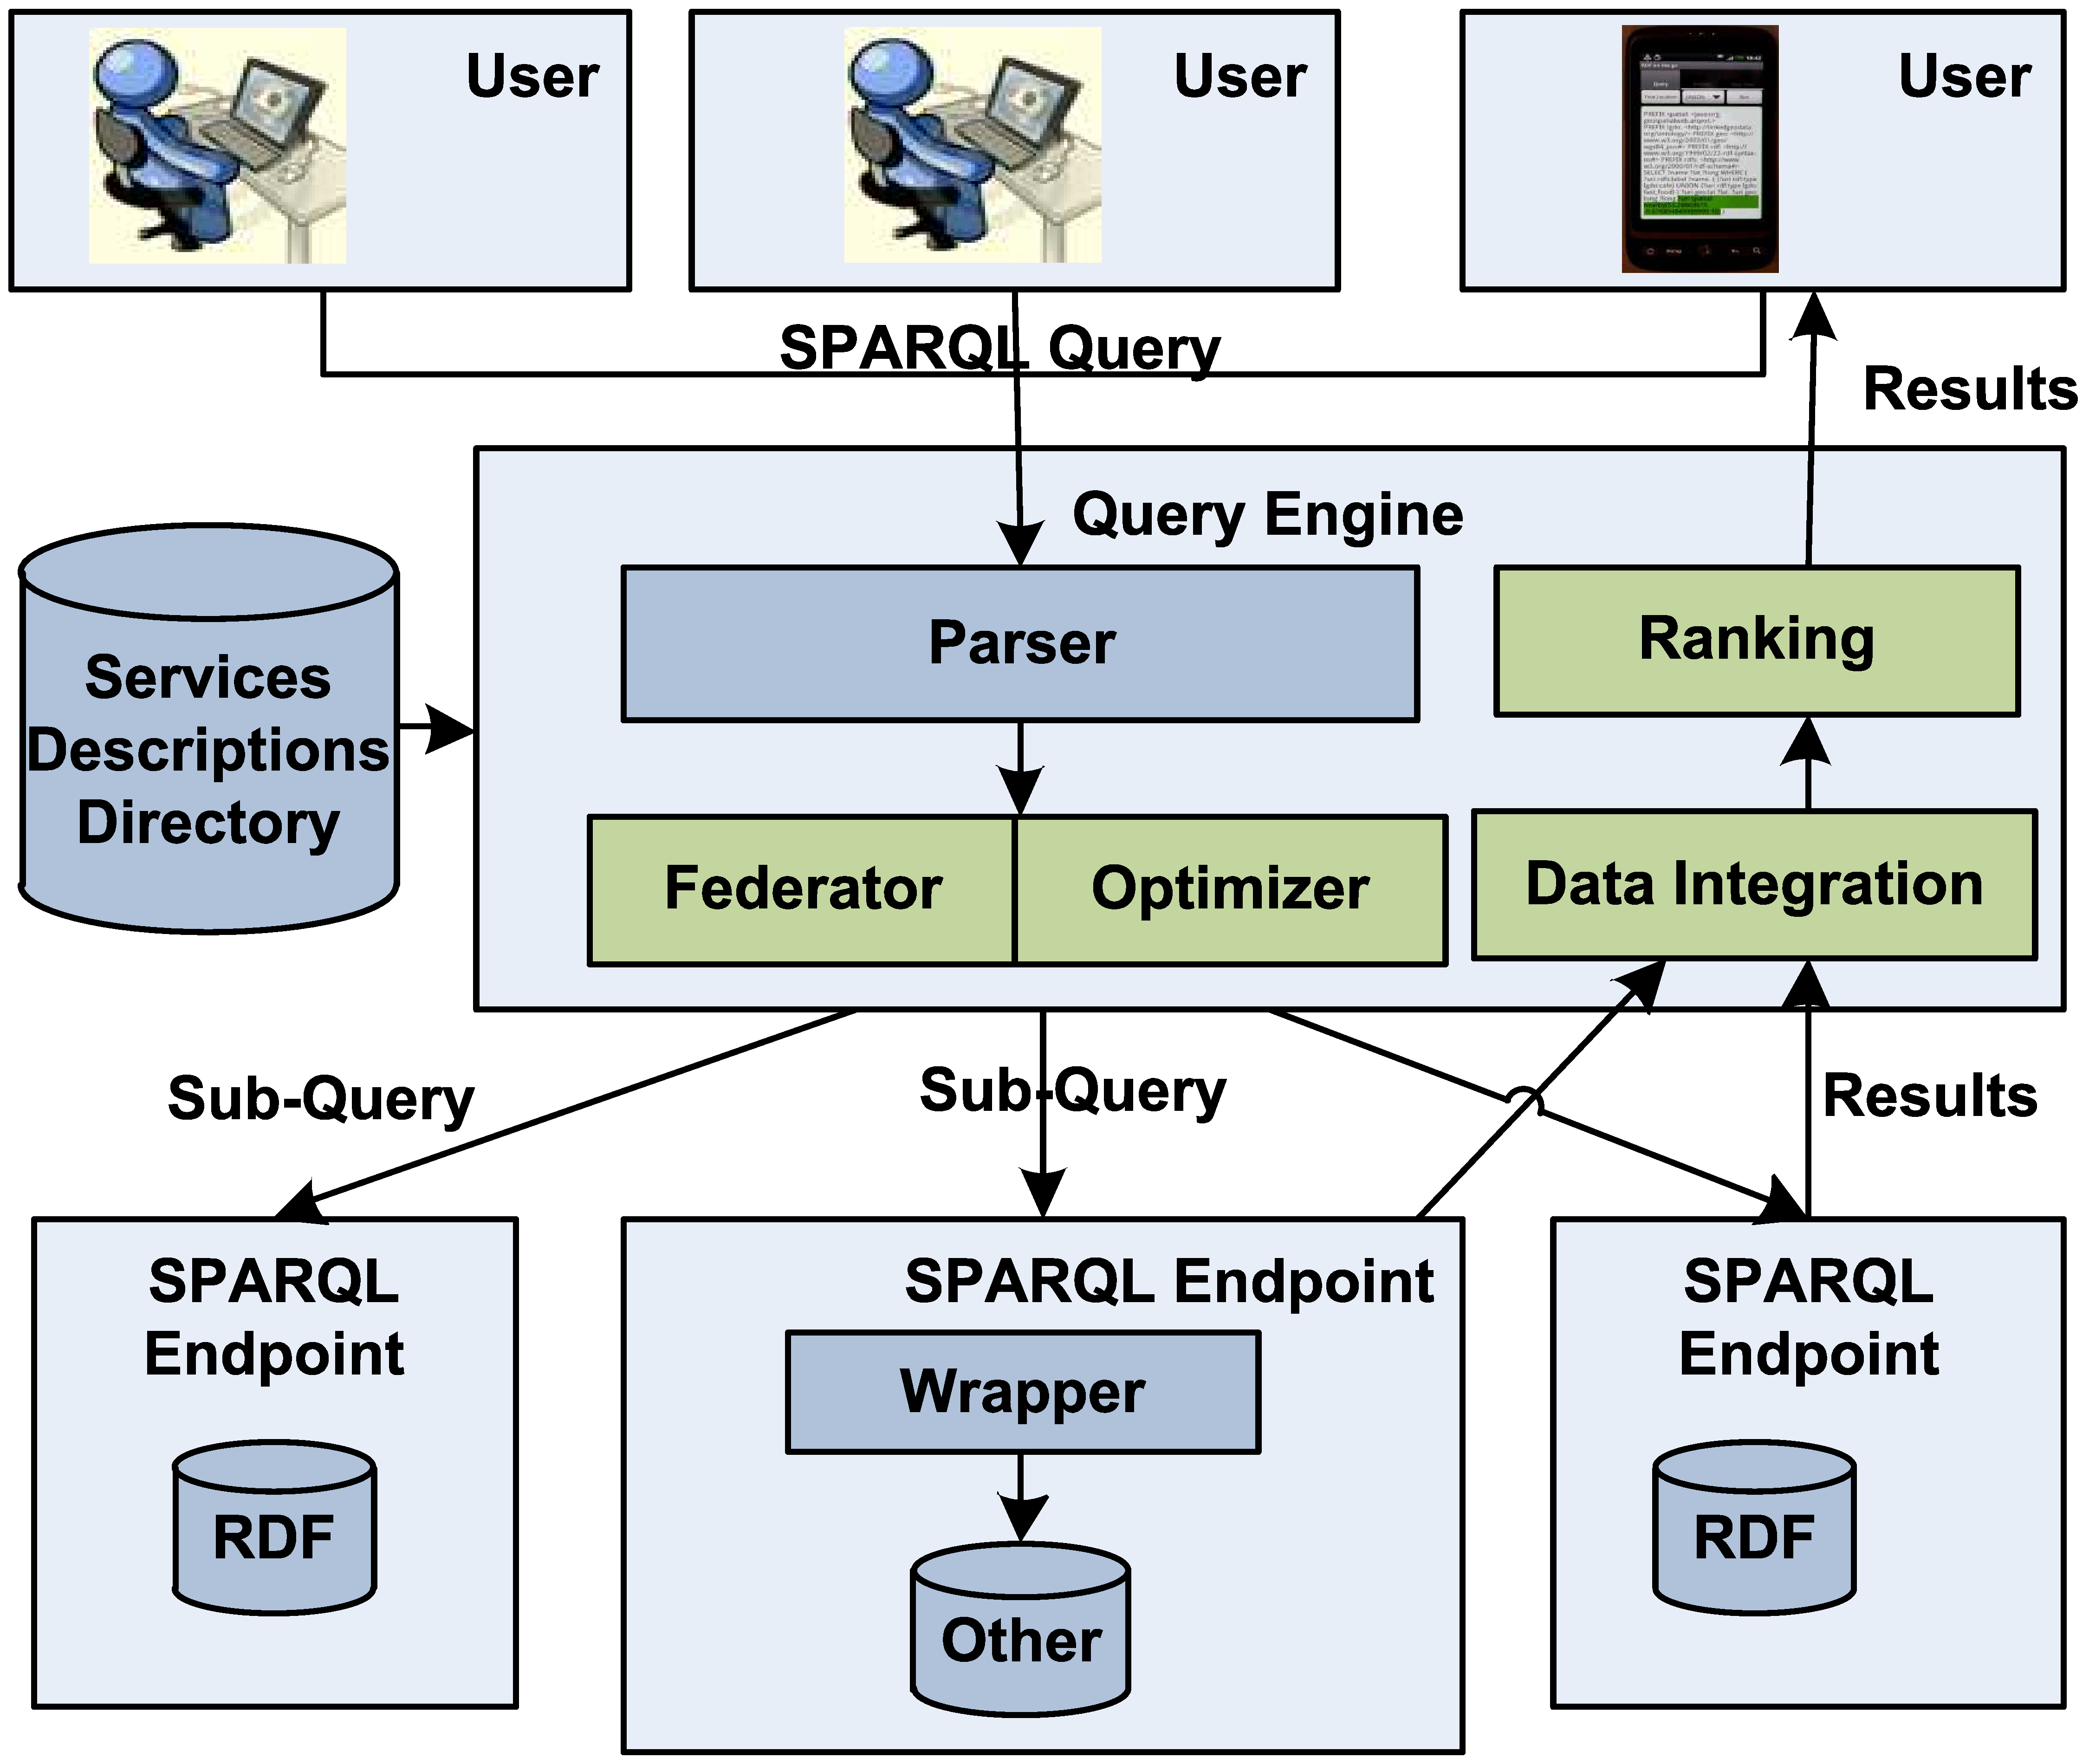
\includegraphics[scale=0.11]{Fig1} 
\par\end{centering}

\centering{}\caption{Federated SPARQL query processing architecture}
\end{figure}
\subsection{MIPS}
Min-Wise Independent Permutations (MIPs) assumes that the set elements can
be ordered (which is trivial for integer keys) and computes N random
permutations of the elements. Each permutation uses a linear hash
function of the form  hi(x) : = ai{*} x + i mod U 
where U is a big prime number and ai,
bi are fixed random numbers. By ordering the resulting
hash values, we obtain a random permutation. For each of the N permutations,
the MIPs technique determines the minimum hash value, and stores it
in an N-dimensional vector, thus capturing the minimum set element
under each of these random permutations. The technique is illustrated
with an example in figure 3 taken from {[}13{]}. Its fundamental rationale
is that each element has the same probability of becoming the minimum
element under a random permutation. By using sufficiently many different
permutations, we can approximate the set cardinality.

An unbiased estimate of the pair-wise resemblance of sets using their
N-dimensional MIPs vectors is obtained by counting the number of positions
in which the two vectors have the same number and dividing this by
the number of permutations N. Essentially, this holds as the matched
numbers are guaranteed to belong to the intersection of the sets.

For a predicate p$\in$ D, the set elements are all triples T $\in$
D with predicate p and computes N random permutations. The resulting
MIP vector is stored against each capability of the service description.
MIP vector statistics is used during source selection and sub-query
generating algorithm for efficient, duplicate free query execution
plan.

\begin{figure}
\begin{centering}
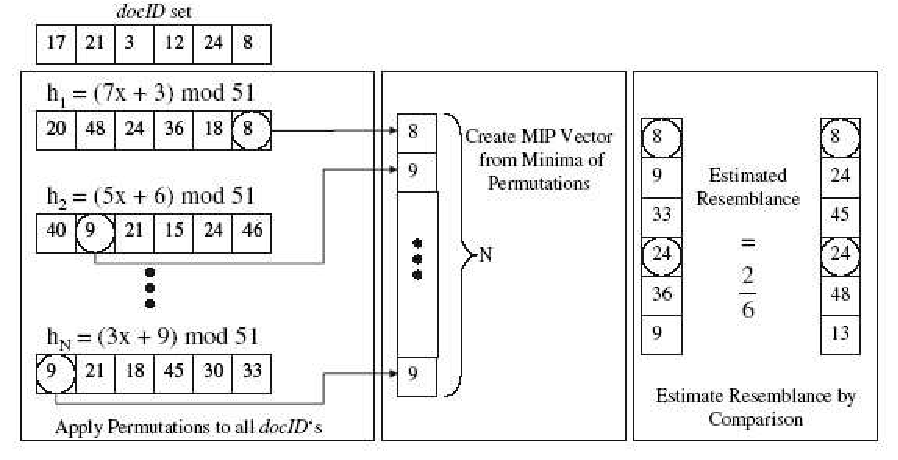
\includegraphics[scale=0.6]{6} 
\par\end{centering}

\centering{}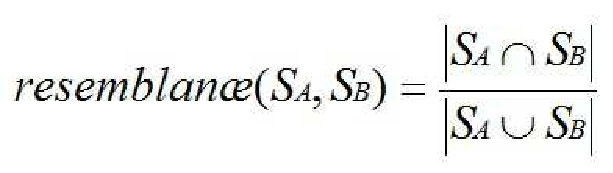
\includegraphics[scale=0.4]{equ}\caption{Min-Wise independent permutations (image taken from {[}13{]} with
permission)}
\end{figure}


\subsection{Index construction}
To find the set of relevant servers and decompose the user query into
multiple sub-queries, the query engine needs information about the
different data sets available at different servers. We call this catalog
the \textbf{service description directory}. Each service description
provides a declarative description of the data available from a server
along with statistical information. The statistical information are
used for query optimization. However, the directory size should be
small enough and must contain sufficient information to enable sub-query
generation, optimization and pre-processing dataset overlap estimation.
Moreover, the directory should be dynamically updated for up to date
data retrieval and accurate overlap detection.

In the initial stage, we only store the\textit{ server url}, and for
each distinct predicate \textbf{p} we record \textit{predicate name,
MIPs Vector,} and \textit{total number of triples} having predicate
\textbf{p}. The MIPs vectors are used to estimate the dataset overlap
before query execution. The other statistical information is used
during sub-query generation and optimization. During this work, we
are planning to use other statistical information such as subject/object
selectivity, histograms, links across the knowledge bases and ontology
matching data. In addition, we will use a mediator to constantly update
the service description directory. A sample service description for
Galway geo data is given in the listing 1.



\subsection{Source Selection}
A SPARQL query contains one or more filtered basic graph patterns
of which each contains the actual triple patterns. The query planning
step is performed separately for each filtered basic graph pattern.
The algorithm used in DARQ for finding the relevant data sources for
a query simply matches all triple patterns against the capabilities
of the data sources. The matching compares the predicate in a triple
pattern with the predicate defined for a capability and evaluates
the constraint for subject and object. Let BGP be a set of triple
patterns in a filtered basic graph pattern. The result of the source
selection is a set of data sources Dj for each triple
pattern.

* need to include the source selection

We extended the DARQ source selection algorithm by comparing different
MIP vectors for similarity. For a triple pattern, we compare the MIP
vectors of all the relevant data sources for possible similarity.
A specific source D is only added to the set of capable sources j,
if D is able to produce new results above a specific threshold value
defined for similarity. For a triple T in dataset D, if the resemblance
value is less than the threshold, D is ignored from set Dj.


\subsection{Source Ranking}
Result set estimation       
\subsection{Subquery generation}
We need an efficient algorithm for sub-query generation using the
service description directory. In the initial stage we are using the
sub-query generating algorithm of DARQ given in figure 2. We represent
a sub-query as triple (T,C, d), where T is a set of triple patterns,
C is a set of value constraints and d is the data source that can
answer the sub-query. Algorithm 1 shows how the sub-queries are generated.
If a triple pattern matches exactly one data source (Di
= \{d\}) the triple will be added to the set of a sub-query for this
data source. All triples in this set can later be sent to the data
source in one sub-query. If a triple matches multiple data sources
the triple must be sent individually to all matching data sources
in separate sub-queries.
\begin{figure}
\begin{centering}
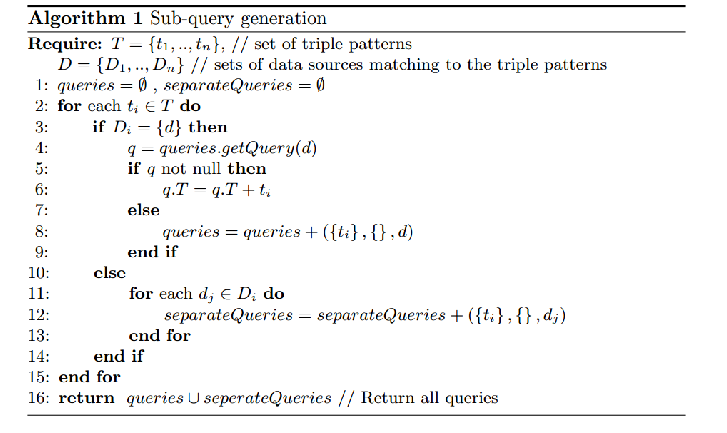
\includegraphics[scale=0.7]{Algo1} 
\par\end{centering}
\caption{Sub-query Generating Algorithm}
\end{figure}

\section{Experiments and Results}
The goal of our experiments was to quantify how well our duplicate-aware solution approximates the result sets from each of the data source from which it can choose and how this approximation affects the way the data sources are ranked.
For this purpose, we compared our approach with two other approaches: DARQ and the optimal duplicate-unaware solution to result set estimation and query ranking. 
In the following, we describe our experimental setup in detail and contrast the results achieved by each of the approaches.
All data used is either publicly available or can be found at the project webpage.\footnote{\url{http://???}}
\subsection{Experimental Setup (AN)}
\subsubsection{Datasets}
Within our experiments, we used the four datasets described in Table \ref{tab:datasets}.
We chose data sets of different data sizes to gain some insights on the scalability of our approach.
The size of the MIPS vectors was set to achieve a compression ratio of approx. 95\% as used in previous work~\cite{QTREE}.
In addition, we emulated the difference between the number of relevant triples across datasets by introducing the discrepancy constant $d$.
Given $n$ data sources of sizes $|S_i|$
\begin{equation}
d = \max\limits_{1 \leq i \leq n} |S_i| - \min\limits_{1 \leq j \leq n} |S_j|.
\end{equation}
Note that the discrepancy accounted for between ca, 1.6\% and 2.8\% of the triples and was to increasingly higher values for increasingly larger data sets.
The number of slices was set to 10 in all experiments.
\begin{table*}
\centering
\begin{tabular}{lrrrrrrrrr}
\hline
Dataset & Size  & Summary 	& CR   & Slices & Discrepancy & Duplicate  & Duplicate & Total 	& Sum. Gen. \\
				& (MB) 	& Size (MB) & (\%) &	  		 &  					 & Slices 		& Datasets 	& Triples & Time (sec)\\
\hline
Diseasome 			& 18.6 	& 1.0 	& 95 & 10 & 1,500 		& 1 & 10 			& 91,122 & 9\\
DBLP 						& 39.0	& 2.8 	& 93 & 10 & 2,500 		& 1 & 10 			& 234,405 & 16\\
Geo Coordinates & 274.1 & 24.4 	& 92 & 10 & 50,000 	& 2 & 				& 1,900,006 & 2705\\
LinkedMDB 			& 448.9 & 41.3 	& 91 & 10 & 100,000 	& 1 & 2 			& 3,579,616 & 3556\\
\hline
\end{tabular}
\caption{Overview of datasets. CR stands for Compression Ratio.}
\label{tab:datasets}
\end{table*}

\begin{table*}
\centering
\begin{tabular}{lrrrrrrr}
\hline
Dataset Name 		& $BGP$  & $S-1$ & $S-2$ & $P-1$ & $P-2$ & $P-3$ & Total \\\hline
Diseasome 			& 5 & 5 & 5 & 4 & 5 & 2 & 26 \\
Geo Coordinates & 5 & 5 & 5 & 0 & 0 & 0 & 15 \\
LinkedMDB 			& 5 & 0 & 0 & 0 & 0 & 0 & 5 \\
Publication 		& 5 & 5 & 5 & 7 & 7 & 4 & 33 \\\hline
Total 					& 20 & 15 & 15 & 11 & 12 & 6 & 79\\
\hline
\end{tabular}
\caption{Distribution of query types across datasets}
\label{tab:queries}
\end{table*}

\begin{table*}
\centering
\begin{tabular}{lrrrrrrr}
\hline
Dataset Name		&BGP 	&S-1&S-2&P-1&P-2&P-3&Total \\\hline
Diseasome				&7		&21	&21	&8	&20	&12	&89\\
Geo Coordinates	&10		&15	&23	&0	&0	&0	&48\\
LinkedMDB				&5		&0	&0	&0	&0	&0	&5\\
Publication			&1		&2	&5	&0	&0	&0	&8\\\hline
Total 					&23		&38	&49	&8	&20	&12	&150 \\\hline
\end{tabular}
\caption{Distribution of query escaped by our approach}
\label{tab:escaped}
\end{table*}


\subsubsection{Queries}
We used three main types of queries. 
Simple basic graph pattern (BGP) queries consisted of exactly one triple pattern in the query.
Star-shaped and path-shaped queries were defined as in~\cite{QTREE}: star-shaped queries (denoted $S-k$) have one variable as subject and contained k triple patterns. 
Path-shaped queries, denoted $P-k$ on the other hand were generated by using a random walk approach to generate a path of length $k$. 
Note that previous work has shown that these query shapes are the most common shapes found in real-world RDF queries~\cite{DPSBM}.
Overall, our benchmark data consisted of 79 queries as shown in Table~\ref{tab:queries}.
Note that some query shapes could not be used on certain datasets due to the topology of the ontology underlying the datasets not being permissive for such queries. 
For example, $S-2$ queries could not be sent to LinkedMDB because 

\subsubsection{Metrics}
We used two measures to compare our approach with the state of the art.
First, we measured the mean squared error of each approach with respect to their result set evaluation as follows:
For each query $q_i$, each source $S_i$ contained a number $R_i(q_i)$ of non-duplicate results.
Each of the approaches generated an approach $\tilde{R}_i(q_i)$ of $R_i(q_i)$.
The mean squared error with respect to the result set size (short $RSMSE$) was then computed as follows:
\begin{equation}
RSMSE = \frac{1}{|Q|}\sum\limits_{q_i \in Q}|R_i(q_i) - \tilde{R}_i(q_i)|^2.
\end{equation}
In addition to the MSERS, we also computed how well the approaches were able to rank the data sources with respect to the unseen triples they would return for a given query.
Given the ideal ranking $rank(S_i, q_j)$ of each data source $S_i$ for each query $q_j$, we computed the mean squared ranking error (short $RankMSE$) of an approach characterized by the the ranking function $\tilde{r}(S_i, q_j)$ by using the following formula:
\begin{equation}
RankMSE (q_j) = \frac{1}{|\mathfrak{S}|}\sum\limits_{S_i}|rank(S_i, q_j) - \tilde{r}(S_i, q_j)|^2.
\end{equation}
\begin{equation}
RankMSE  = \frac{1}{|Q|}\sum\limits_{q_j  \in Q}RankMSE(q_j).
\end{equation}
For both measures, higher values are obviously worse.


\subsection{Results}
The RSMSE results are shown in Figures~\ref{fig:rsmse} while the ranking results are shown in Figure~\ref{fig:rank}.
In each figure, we compared the results of the approaches w.r.t. both the whole input query and to each of the triples patterns contained in the input queries.
The RSMSE results are shown on a logarithmic scale, meaning that 
Our results clearly show that we outperform the state of the art w.r.t to both result set estimation and ranking. 

\begin{figure}
\centering
\begin{subfigure}[b]{0.45\textwidth}
                \centering
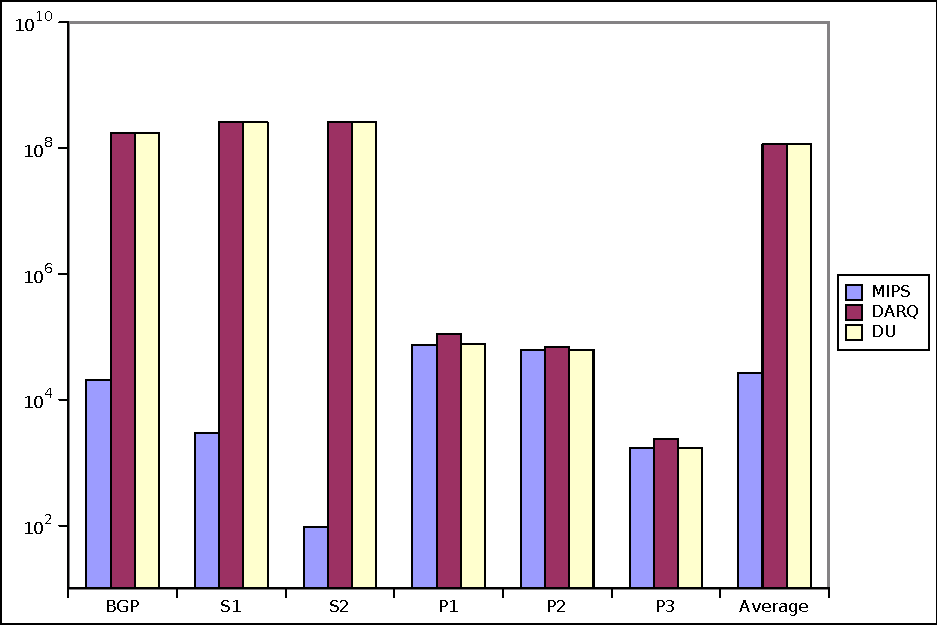
\includegraphics[width=\textwidth]{img/querywise_rse}
                \caption{RSMSE for query-wise selection (vertical log scale)}
                \label{fig:rsmsequery}
        \end{subfigure}
\begin{subfigure}[b]{0.45\textwidth}
                \centering
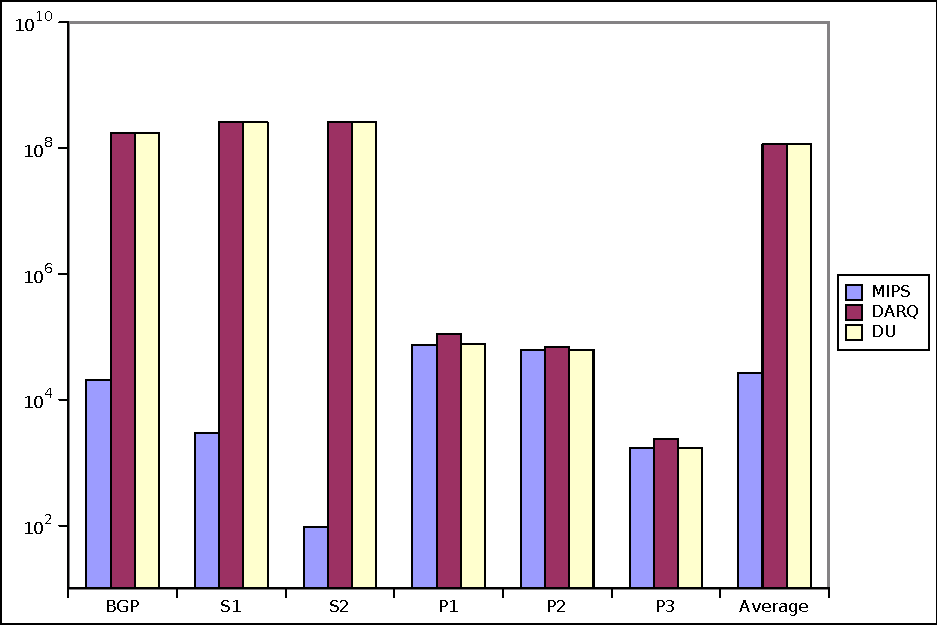
\includegraphics[width=\textwidth]{img/subquerywise_rse}
                \caption{RSMSE for subquery-wise selection (vertical log scale)}
                \label{fig:rsmse_subquery}
        \end{subfigure}
\caption{Mean squared errors with respect to result set evaluation}
\label{fig:rsmse}
\end{figure}

\begin{figure}
\centering				
\begin{subfigure}[b]{0.45\textwidth}
                \centering
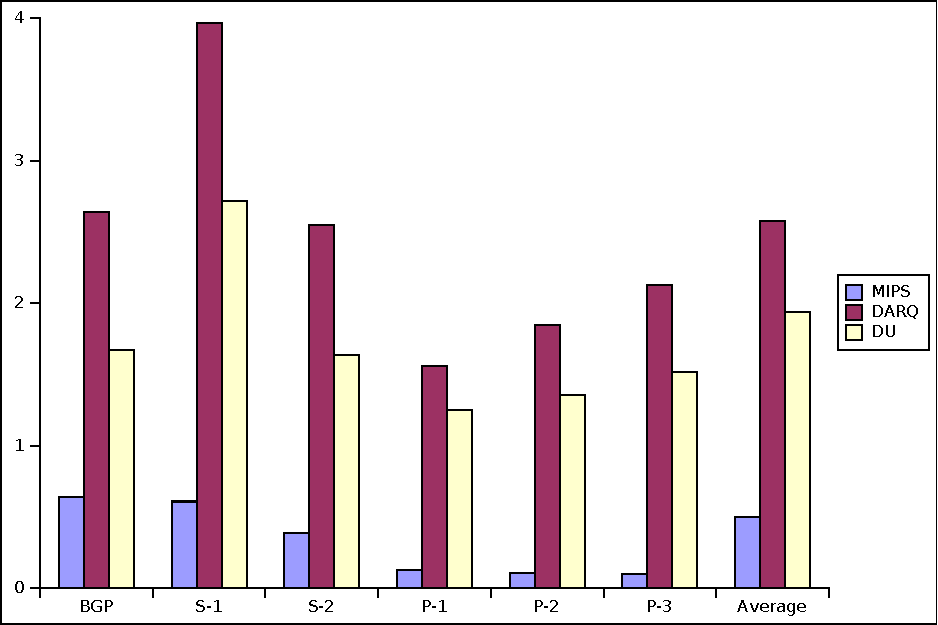
\includegraphics[width=\textwidth]{img/querywise_ranking}
                \caption{RankMSE for query-wise selection}
                \label{fig:rankmsequery}
        \end{subfigure}				
				\begin{subfigure}[b]{0.45\textwidth}
                \centering
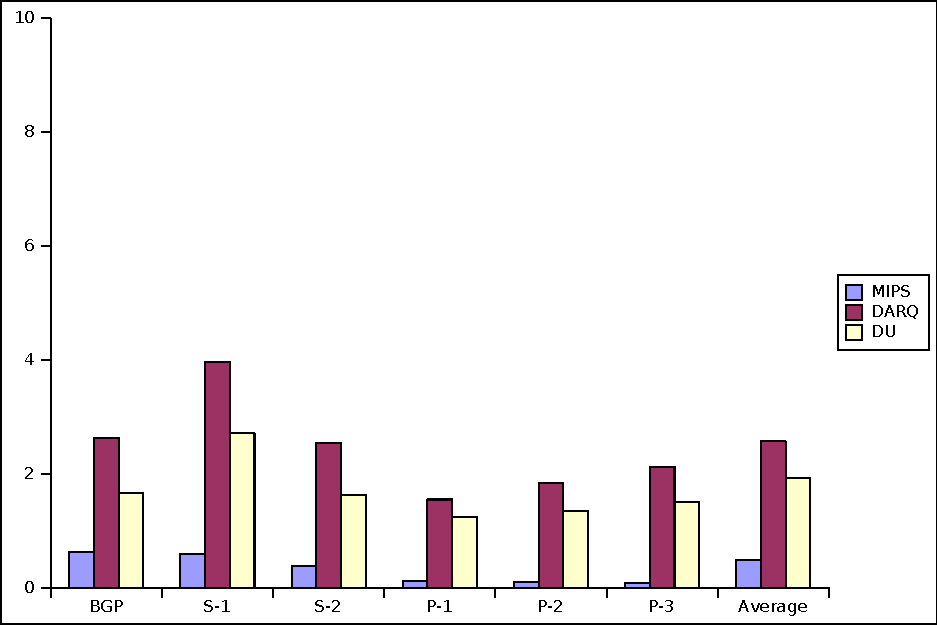
\includegraphics[width=\textwidth]{img/subquerywise_ranking}
                \caption{RankMSE for subquery-wise selection}
                \label{fig:rankmse_subquery}
        \end{subfigure}
\caption{Mean squared errors with respect to ranking}
\label{fig:rank}
\end{figure}

\subsubsection{Ranking Error}
\subsubsection{Result Set Estimation Error}
\subsubsection{Execution Time}
\subsubsection{Size of MIPS vectors (on largest dataset)}
\section{Discussion (AN)}



%\bibliographystyle{plain}
%\bibliography{literature}
\begin{thebibliography}{10}
\bibitem{key-1}Stuckenschmidt, H., Vdovjak, R., Houben, G.J., Broekstra,
J.: Index structures and algorithms for querying distributed rdf repositories.
In: WWW'04. (2004).

\bibitem{key-2}Quilitz, B., Leser, U.: Querying distributed RDF data
sources with SPARQL. In: European semantic web conference on the semantic
web: research and applications (ESWC 2008). LNCS, vol. 5021, pp. 524-
538. Springer, Heidelberg (2008).

\bibitem{key-3}Langegger, A., Waoay, W., Blaochl, M.: A semantic web
middleware for virtual data integration on the Web. In: European semantic
web conference on the semantic web: research and applications (ESWC
2008). LNCS, vol. 5021, pp. 493-507. Springer, Heidelberg (2008).

\bibitem{key-4}Hartig, C. O, Bizer, J.-C. Freytag. Executing SPARQL
queries over the web of linked data. 8th International Semantic Web
Conference (ISWC 2009).

\bibitem{key-5}Harth, A., Hose, K., Karnstedt, M., Polleres, A.,
Sattler, K.U. Umbrich, J.: Data summaries for on- demand queries over
linked data. In: (WWW 2010), USA.

\bibitem{key-6}Umbrich, J., Hose, K., Karnstedt, M., Harth, A., Polleres.:
Comparing data summaries for processing live queries over Linked Data.
In:(WWWJ 2011), special issue querying the data web. 

\bibitem{key-7}Schwarte, .A, Haase, .P, Hose, .K, Schenkel, R, Schmidt,
M.: FedX: Optimization Techniques for Federated Query Processing on
Linked Data. In: 10th International semantic web conference (ISWC
2011).

\bibitem{key-8}Perez, J., Arenas, M., Gutierrez, C.: Semantics and
Complexity of SPARQL. In: 4th International SemanticWeb Conference
(ISWC), Athens, GA, USA (November 2006).

\bibitem{key-9}Broder, A. Z., Charikar, M., Frieze, A. M., \& Mitzenmacher,
M. (2000). Min-wise independent permutations. Journal of Computer
and System Sciences, 60(3), 630-659.

\bibitem{key-10}Bloom, B. H. (1970). Space/time trade-offs in hash
coding with allowable errors. Communications of ACM, 13(7), 422-426.

\bibitem{key-11}Mitzenmacher, M. (2002). Compressed bloom filters.
In IEEE/ACM Transactions on Networking, 10(5), 604-612.

\bibitem{key-12}Bender, M., Michel, S., Weikum, G., \& Zimmer, C.
(2005). Minerva: Collaborative p2p search. In Proceedings of the (VLDB)
conference (Demonstration).

\bibitem{key-13}Parreira, J.X, Michel, S., Weikum, G.: p2pDating:
Real life inspired semantic overlay networks for Web search. In: Journal
of Information Processing and Management 43 (2007) 643-664.

\bibitem{key-14} http://www4.wiwiss.fu-berlin.de/lodcloud/state/

\bibitem{key-15}Y. Li and J. Hefl{}in. Using reformulation trees
to optimize queries over distributed heterogeneous sources. In ISWC,
pages 502-517, 2010.

\bibitem{key-16}Z. Kaoudi, K. Kyzirakos, and M. Koubarakis. Sparql
query optimization on top of dhts. In ISWC, pages 418-435, 2010.

\bibitem{key-17}A. Deshpande, Z. G. Ives, and V. Raman. Adaptive
query processing. Foundations and Trends in Databases, 1(1):1-140,
2007.

\bibitem{key-18} G. Ladwig and T. Tran. Linked data query processing
strategies. In ISWC, pages 453-469, 2010.

\bibitem{key-19}G. Ladwig and T. Tran. Sihjoin: Querying remote and
local linked data. In ESWC (1), pages 139-153, 2011.

\bibitem{key-20}Auer.S, Lehmann. J, Ngonga, A.C.: Introduction to
Linked Data and Its Lifecycle on the Web. In: Reasoning Web. Semantic
Technologies for the Web of Data, Pages 1-75, 2011.

\bibitem{key-21}M. Acosta, M.-E. Vidal, T. Lampo, J. Castillo, and
E. Ruckhaus. Anapsid: An adaptive query processing engine for sparql
endpoints. In Proc. of International Semantic Web Conference (ISWC),
2011.

\bibitem{key-22}C. Buil-Aranda, M. Arenas, and O. Corcho. Semantics
and optimization of the sparql 1.1 federation extension. In ESWC (2),
pages 1-15, 2011.

\bibitem{key-23}. M. Stoker, A. Seaborne, A. Bernstein, C. Keifer,
and D. Reynolds. SPARQL Basic Graph Pattern Optimizatin Using Selectivity
Estimation. In WWW, 2008.

\bibitem{key-27}C. Basca and A. Bernstein. Avalanche: Putting the
Spirit of the Web back into Semantic Web Querying. In The 6th International
Workshop on SSWS at ISWC, 2010.

\bibitem{key-28}O. Hartig. Zero-knowledge query planning for an iterator
implementation of link traversal based query execution. In ESWC, pages
154-169, 2011.

\bibitem{key-29}Axel-Cyrille Ngonga Ngomo and Soren Auer. LIMES -
A Time-Ecient Approach for Large-Scale Link Discovery on the Web of
Data. In Proceedings of IJCAI, 2011.

\bibitem{key-30} R. Isele, A. Jentzsch, and C. Bizer. Ecient Multidimensional
Blocking for Link Discovery without losing Recall. In WebDB, 2011.

\bibitem{key-31}Axel-Cyrille Ngonga Ngomo and Klaus Lyko. EAGLE:
Ecient Active Learning of Link Specications using Genetic Programming.
In: ESWC(2012).

\bibitem{key-32}Unger, C.; Buhmann, L.; Lehmann, J.; Ngonga Ngomo,
A.-C.; Gerber, D.; and Cimiano, P. Templatebased question answering
over RDF data. In WWW (2012).

\bibitem{key-33}G.Koutrika, and Y.Ioannidis, Personalized Queries
under a Generalized Preference Model, In ICDE 2005.

\bibitem{key-34}G.Koutrika, and Y.Ioannidis, Personalization of Queries
in Database Systems, In ICDE 2004.

\bibitem{key-35}S.Magliacane, A. Bozzon.E.D. Valle. Efficient Execution
of Top-k SPARQL Queries. In: ISWC(2012), USA. 

\bibitem{key-36}B. J. Frey and D. Dueck. Clustering by passing messages
between data points. Science, 315:972-976, 2007.

\bibitem{key-37}{]} V. Levenshtein. Binary codes capable of correcting
deletions, insertions, and reversals. In Soviet Physics Doklady, volume
10, 1966.

\bibitem{key-38}M. Morsey, J. Lehmann, S. Auer, and A.-C. {Ngonga Ngomo}.
DBpedia SPARQL Bench- mark - Performance Assessment with Real Queries
on Real Data. In 10th Interna- tional Semantic Web Conference (ISWC2011),
2011\end{thebibliography}

\end{document}
